\chapter{Interactive Musical Score}

\section{Introduction}

Learning to read music from the score is an essential part of Western classical music
training. Traditionally, children learn the different music notes by singing or playing
notes on an instrument, guided by a teacher. We envision a way for children to learn
the correspondence between notation and sound by directly touching the score.
The Interactive Score is effortless to use and allows children to make discoveries on
their own. The correspondence between the visual, the tactile, and the sound can aid
in learning.

In this work, we introduce the Interactive Score, a novel instrumental device for children's solfege
learning. Paper scores are overlaid onto a staff drawn with conductive ink and
connected to an Adafruit musical box. Pressing a note in the score triggers its sound,
and running fingers over the notes plays a melody.


\subsection*{Motivation}

\section{Related work}

\subsection{Context} 

A review of music theory pedagogy over the past decade reveals many criticisms of the way music theory courses have been taught. Other concerns include issues such as whether to take a harmonic, melodic, or compositional approach to teaching theory. The early involvement of students in creative thinking about harmony, melody, and rhythm determines in part its success in the theoretical program \cite{bland1977college}. The development of a feeling for the mastery of the preliminaries to music as well as the presentation of the basics are the prerequisites for a successful future theoretical education.

But out of the large number of students who embark on learning music, only a small portion retain the courage and motivation to continue their studies to the end.
For example, out of 100 French people aged 15 and over, a study recorded that only 30\% of the musicians who have learned music continue to practice their instrument during their their lives \cite{amateurs}. 

It is pointless and frustrating for students to be pushed too quickly into advanced and sophisticated theory without visualizing audibly what they are studying.

\subsection{Approaches}

Music theory courses can take many forms. There are many approaches to developing musicianship skills. Teachers often choose between traditional or more contemporary approaches.

\paragraph*{Traditional approach}

Traditional music lessons prepare students to read, write and perform music from the work of great academic composers. It produces excellent results in terms of sight-reading skills. But a significant number of students leave these music studies because of their lack of enjoyment of the method.


\paragraph*{Contemporary approach}
Contemporary music lessons are paired with instrumental lessons (usually piano or guitar). They do not require music reading or theory. These lessons focus on skill, musicality, and more intuitive learning methods. They require the student to have a good ear for music and a sense of rhythm. The contemporary approach is beneficial for students who have difficulty visualizing with theory classes. They are able to play real pieces only a few months after starting their lessons.  


The actual major advice if a student has any problem understanding music theory, is to study the theory on the piano. Intervals and harmonies are easier to understand on a piano first, as is all the rest of the theory.

\subsection{Musical Mental Projection}

Musical imagery, or the ability to create an image of sound in our minds, is an essential
skill for all musicians. For example, brass, winds, strings, and singers imagine the
pitch of an upcoming note to make it easier to play it and determine the distance from
the previous note
\cite{zatorre2005mental}. Composers and arrangers also use musical imagery when creating
a new piece. Musical imagery training has been shown to improve the ability to follow
the upward and downward movements of the tonal contour of a musical phrase or
imagined tune
\cite{weber1986musical}.

Ear training" (or solfege) has traditionally been part of the curriculum of most music
schools. An important part of solfege is the ability to read music notation and imagine
how it is supposed to sound. We are interested in teaching this skill to children.


\subsection{Tangible Interactive Medias for Music Practise}

Many projects aim at getting a child involved in the world of music. For example, Zigelbaum et al. investigated how electronic instruments can engage young learners in learning to make music. Their project was the development of different tools involving movement, linking it to a sound. They created a trampoline, an interactive matrix, or musical bracelets \cite{zigelbaum2006bodybeats}.

Some projects related to interactive scores already exist. But their development just aims for the design and performance of Electroacoustic music \cite{struc_inter_music_score} and live spectacles. The primary goals of such scores are to develop a computer-aided composition environment allowing the composer to create such interactive scores and a performance machine making their interpretation possible.

"MixMatrix" sheet of push-pads

An excellent example of a project was Xio Xio et Al. one, which provides an understanding of the essential workings of music without going into the details of music theory \cite{xiao2014andante}.

\begin{marginfigure}
    \centering
    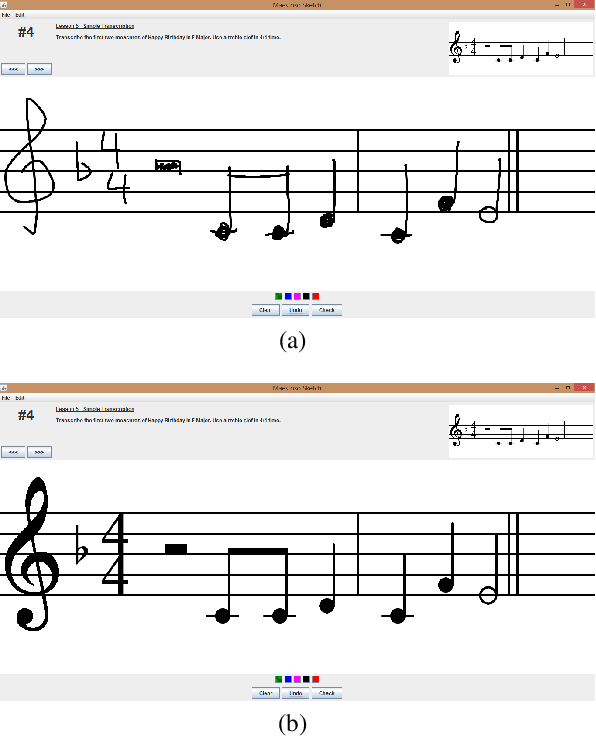
\includegraphics{images/maestoso.png}
    \caption{Maestoso Educational
    Sketching Tool for Learning Music Theory}
    \label{fig:taele2015maestoso}
\end{marginfigure}

The work of Taele et al. \cite{taele2015maestoso} \ref{fig:taele2015maestoso} describes the practical and cognitive benefits of learning music theory for both musicians and non-musicians. The paper proposes an intelligent educational tool designed to help students learn music theory. The tool, called Maestoso, utilizes sketch-based interaction and machine learning techniques to provide personalized feedback to the user.
The paper first introduces the importance of music education and the challenges students face when learning music theory, such as the abstract nature of music concepts and the difficulty of translating musical ideas into notation. The authors argue that sketching could be an effective approach to help students overcome these challenges and propose Maestoso as a solution.
Maestoso is based on a sketching interface that allows users to draw musical notes, chords, and melodies using a stylus or finger. The program uses machine learning algorithms to recognize the user's sketches and provide feedback on their accuracy and completeness.

Implementing such systems is often fully digital and interactive through a screen. Some projects aim to teach children music theory or interact with notes to compose, learn and experiment. Most of these projects are applications that users can download on smartphones or tablets. The relationship with the tangible paper score is gradually lost and will soon be entirely replaced by digital interaction.

One solution is to use conductive ink to keep a tool in paper form without losing its interactive aspect. Conductive inks, paints, and varnishes are liquids containing metal particles, conductive polymers, or graphite. They are specifically designed to conduct electricity.

Inkjet printing has been used to pattern organic semiconductors \cite{kim2008heterogeneous}, metal contacts on organic semiconductors \cite{khan2019soft} \cite{wessely2020sprayable}, and metallic structures that require minimal further processing. Researchers such as Ahn et al. used conductive ink printing to realize metallic connections between functional components of flexible devices. Another project like that of Russo et al. has resulted in an optical image of a flexible paper display containing a LED array. It takes the form of a multi-color 25 × 16 LED array connected to the printed silver electrodes by depositing a drop of concentrated silver ink \cite{russo2011pen}.

\section{General Architecture}

\subsection{Overview}

Online many digital music learning applications, which run on screen-based devices,
our design augments a traditional paper score. Children already spend a considerable
time in front of screens, which can harm their eyes from a young age. Paper is flexible,
lightweight and easily transportable, and the incorporation of electronic circuits in
paper has shown its attractiveness to children
\cite{hershman2018light}.

\begin{figure}[h]
    \centering
    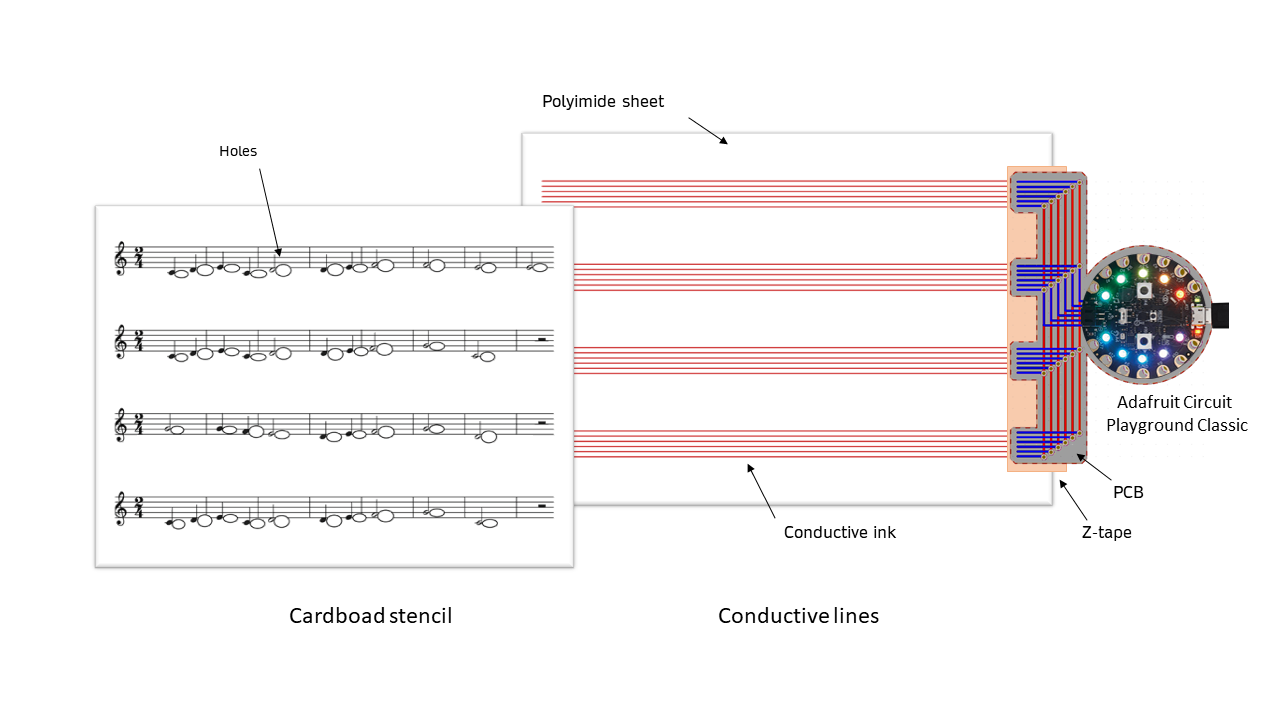
\includegraphics{images/IS_schema.png}
    \caption{Interactive Musical Score architecture.}
    \label{fig:IS_schema}
\end{figure}

The demonstrator supplies the electronic part (substrate and PCB) during the
showcase. He places a partition (a cardboard stencil) on top of the substrate (where
the conductive lines are located). He plays the music and then changes it to another
one

\subsection{System Design}

The Interactive score consists of two thin layers. The first layer is the traditional sheet
music, printed on cardstock paper, with holes punched for each note. Under this sheet
is a polyimide substrate with conductive lines printed on it. 
The conductive lines are connected to an Adafruit Circuit Playground printed circuit
board (PCB) using double-sided “z-tape.”
When the user touches a note on the top layer, contact is made between the finger and
the conductive lines through the holes in the cardstock. The signal travels through the
ink paths and the z-tape to the PCB, which detects a potential difference using
capacitive touch and plays the relevant note. The detection of several simultaneous
signals on multiple pins allows the playing of eleven different notes with only six lines.

% TODO Justifier les choix techniques

\subsection{Electronic Music Box}


\begin{marginfigure}
    \centering
    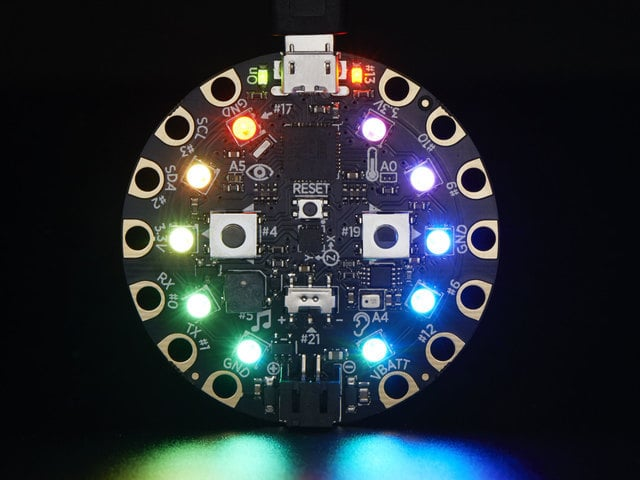
\includegraphics{images/circuit_playground_classic.jpg}
    \caption{Adafruit Circuit Playground Classic}
    \label{fig:circuit_playground_classic}
\end{marginfigure}

The whole system is kept in a 3D printed case, maintaining contact between the polyimide, the z tape, and the PCB.

The signal is recovered and used in capacitive touch with an Adafruit Circuit Playground Classic. An Arduino program allows to generate a vast number of different notes. The code is retrievable on GitHub \cite{adrien2022capacitive_to_notes}.

% TODO Justifier les choix techniques

\subsection{Paper Score Manufacturing}

For perfect dimensional compatibility between the different elements of the score, The music score printed on the stencil was entirely designed in photoshop. Notes, staves, lines, hyphenation, and cutouts were all placed on the same project. It allows the elements to fit together perfectly and export the cutout locations at the correct size relative to the partition's rest.

An inkjet printer draws all cardboard lines, hyphenation, notes, and numbers.

A score of "J'ai du bon tabac" (on the left) is positioned on the substrate. Then, the notes were isolated in another PNG file, selected on Cricut design, and cut directly into the cardboard with Cricut maker 3 (on the right).

% TODO Justifier les choix techniques

\subsection{Conductive Sheet Manufacturing}

The conductive ink lines paths are 1mm thick, 5cm in length, with a resistance of 0.07 Ohms. The lines are printed using a simple inkjet printer equipped to print with silver nanoparticules conductive ink. The printed patterns are then sintered at 180°C for 73 minutes. This process allows the quick production of flexible circuits \cite{khan2019soft}.

This prototype comprises four staffs of 6 lines made of conductive ink on a Kapton polyimide sheet substrate. This polymer does not melt at high temperatures and has excellent mechanical strength, and is very dimensionally stable and creep resistant at temperatures above 260°C. The lines are 1mm thick, and at a distance of 15cm in length, it gave a resistance of 0.07 Ohms.

%TODO Mettre une photo du sheet  
% \begin{figure}[h]
%     \centering
%     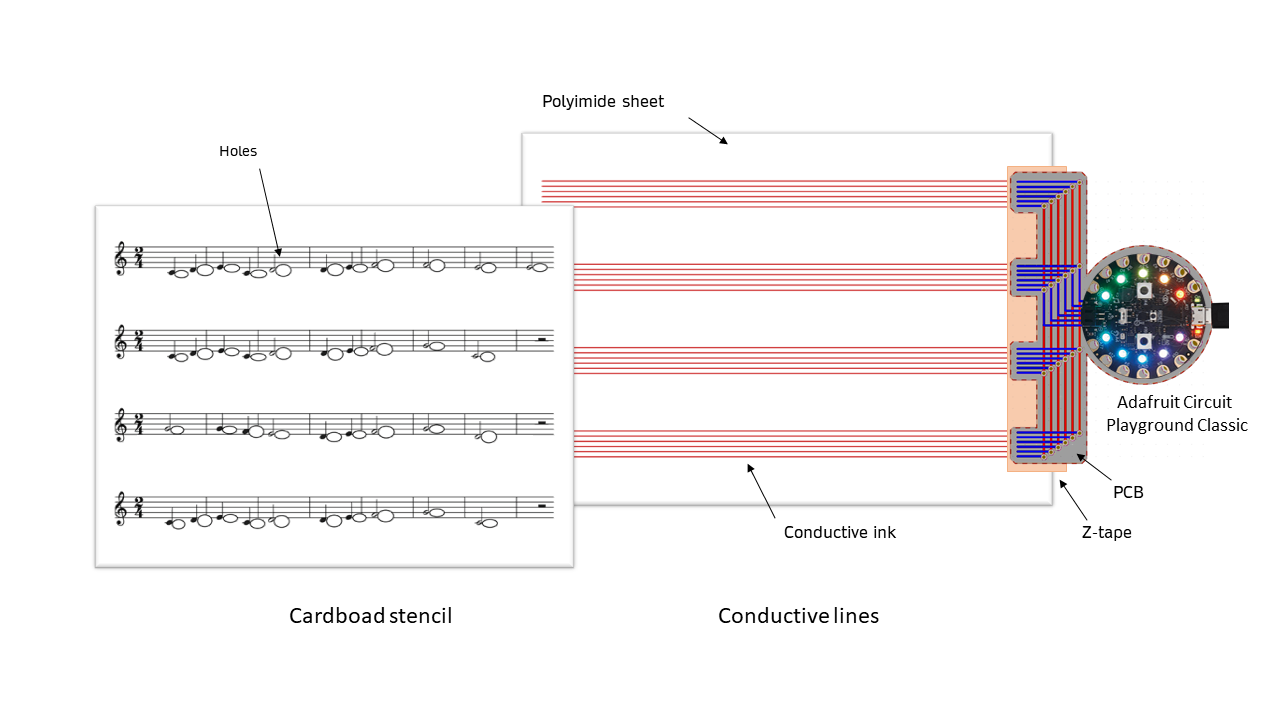
\includegraphics{images/IS_schema.png}
%     \caption{Interactive Musical Score architecture.}
%     \label{fig:IS_schema}
% \end{figure}

An Epson WF-2010 printer printed the lines on the substrate \cite{adrien2022capacitive_to_notes}.

% TODO Justifier les choix techniques

\subsection{Integration and Usability}

\subsubsection{Ability to change the score}

Its ease of interchangeability characterizes the paper score. It is easy to produce. It
can easily be removed from the box and another one placed in its place to play a
different melody. All the electronic parts (substrate, PCB, microcontroller) are
independent of the paper score. The user can change it without changing the code or
the rest of the device. The sheet music has the exact dimensions of the substrate.
Therefore, it is simple to place the two precisely on top of each other to align the
holes with the ink lines.

\subsubsection{Ability to improvise} 

The user has the capacity to improvise by not playing the notes in the same order.
The project allows a great deal of modularity in its use. Just by touching specific
notes at certain times, users can experiment with different rhythms and melodies
and reconstruct a piece from a few notes.
With a simple score including an ascending scale, he can try his hand at composition.
As the microcontroller code is configured to play melodies in C major, it is not
possible to create dissonance.


\section{Applications and Evaluation}

\subsection{Set up}

Four users are selected at random. They interact with the prototype already prepared for use. They then answer several questions. The project is plugged in and set up as a base for further use. The users have tested the prototype. The project does not aim to teach a user how to play music. It seeks to link music theory directly with music practice without requiring knowledge.
It is difficult to test whether the project impacts the user's ability. Therefore, measuring the openness and visualization of music theory given by the project to the user is interesting. The questions concern understanding use, practicality, interest, innovation, attractiveness, and playfulness.

\subsection{Results}

The users did not encounter any particular problems during the test. The prototype worked well. The testers gave interesting feedback. As most of their comments have been taken into account since the last test, there were far fewer negative comments.

The users proposed many ideas to make the project evolve. They advised adding indications, potentially with LEDs, to indicate actions to be carried out. One idea was to create a binder with different stencils inside. They would have appreciated a correction of the electronics, which would warn them if they made a mistake. The people who tested the project were quite satisfied. They liked the fact that they could interact. The fact that the person playing presses the right notes and not that the sound automatically adapts to what they are doing was emphasized. It is because the sounds are corrected to play the right notes on some music toys, wherever the user presses (on the notes of a keyboard, for example). The users were also very interested in the fact that the project is portable. They would have liked to be able to take it with them to play music everywhere.

\section{Discussion}

\subsection{Attractivity}

The project is attractive for children as a tangible object. 
Its gamified aspect makes it close to a toy. This contributes to its attractiveness, especially to young children. Its musical property favors the creativity of the user, in addition to being portable, tactile, fun, and easy to use. 

\subsection{Musical Imagery learning}

An important aspect of musical practice is the ability of the musician to decipher a score. When this one practices with a visual support, his brain must take the exercise to connect the note which he links visually with the position of his fingers on the instrument. An intermediate used by the brain is the transcription of the note read, in its "mental", from which an interval and therefore a position is deduced. The ability to translate the visual note into a sound is therefore a reflex to be trained and very relevant in the practice of music. The basics of this ability must be acquired very quickly when learning the basics of music.

\subsection{Mobilising multiple intelligences}

This kind of device has a real interest in terms of learning. The user practices bodily intelligence with touch, the visual intelligence since he has a support in front of him, but also the musical-rhythmic intelligence.

\section{Conclusion}

In conclusion, the interactive score project has a bright future ahead of it, as it implements a very recent technology to popularize it. This process could be industrialized and even replicable for individuals, with some improvements and optimizations. In the future, our goal is to make the score more accessible. Features such as flexibility and simple "plug and play" aspect make it attractive even to children.

\subsection{Limitations}

%Problème en terme de nombre de notes jouables. Problème en terme de taille de la partition. Problème en terme de son du à l'électronique utilisée. Problème du au scotch conducteur pouvant s'abimer et provoquer des faux contacts. Le courant n'étant plus transmis à travers les lignes. Problème du à l'encre conductrice pouvant s'effriter, empecher le courant de traverser certaines lignes. Problème de superposition du papier par dessus la feuille de polyimide pour aligner les notes avec les lignes d'encre tout en gardant un système flexible. Problème majeure de sensibilité au champ électrique du à l'utilisation du capacitivé touch. A proximité de champs électriques, le microcontrôleur peut détecter des faux contacts. L'appareil est donc à utiliser à distance d'appareils électroniques ainsi que de surfaces métaliques.

\subsection{Future works}

A "musical tutorial" mode will soon be added so that the user can listen to the score's
music before having to play it. This will allow the user to assimilate the musical rhythm
(the time between playing each note) with the physical rhythm (the time between
pressing notes).
The electronic PCB/microcontroller part will be redesigned to no longer integrate an
Adafruit Circuit Playground but a much smaller circuit entirely made by us. The
learner can replace each component in case of a problem. It will be possible to
improve the speaker's quality and connect the device to Bluetooth or Wi-Fi to play
music at a distance.
We are currently looking for partnerships in children's education to research
experimentations on the impact of this interactive score on music assimilation. Several
parameters would be evaluated, such as the concentration level, playing time, and
knowledge retention. We will consider different strategies to transcript musical-rhythmic on this interactive score.